
\documentclass{article}

\usepackage{hyperref,url,booktabs,amsfonts,nicefrac,microtype,amsmath,amssymb,mathtools,xcolor,graphicx,float,fancyhdr,listings}

\title{CS205 Final Project: Teleporting Parallel MCMC}

\begin{document}

\maketitle

\section{Introduction}

Many of the biggest science applications running today -- from climate models
\cite{climate} to economic forecasting \cite{forecast} to experimental physics
\cite{physics} -- are probabilistic simulations. Because the models involved
are often too complex to integrate analytically, these models generally rely on
Monte Carlo methods (basically, drawing lots of samples and taking averages) to
make predictions. But even sampling from these simulations can be challenging.
To do big science, practitioners must not only contend with increasing data
size but also increasing problem complexity.

A specific complexity we are concerned with here (related to the familiar idea
of non-convexity) is multimodality. When a probabilistic simulation is
multimodal, there isn't a single cluster of likely configurations centered
around a characteristic average. Instead, there are multiple such clusters
distributed far away from each other in the model's parameter space. One
example where this occurs is topic modeling \cite{topicmodes}, and also in the
problem of localizing sensors based on noisy measurements of inter-sensor
distance -- which is commonly used as a benchmark for multimodal sampling
techniques \cite{wormhole}, \cite{darting}.

In this project, we will consider how parallelism can help us deal with
problems of big statistical complexity that arise in such applications. We will
also introduce a novel method for efficiently sampling from multimodal
distributions, analyze its scaling properties, and present our implementation
using state-of-the-art parallel computing technologies.

\section{Background}

\subsection{Markov-Chain Monte Carlo (MCMC)}

MCMC is a \textit{local} method for sampling from distributions $s(x)$. One of its
simplest forms is the Metropolis-Hastings algorithm, which works as follows.
Assuming you begin at a point $x_1$, you then propose a point $x_2$ by
sampling from a symmetric proposal distribution $p(x)$. You then either
move there or stay put, and add your current location to the sample chain. The
important point is that the ratio of probability of transitioning from
$x_1$ to $x_2$ and back again must equal the ratio of the target
densities $s(x_1)$ and $s(x_2)$. If this condition (called "detailed
balance") holds, then the sample chain will converge to the true distribution.

Pseudocode for this algorithm is: 

\begin{lstlisting}[mathescape=true]
function MetropolisHastings($s$, $p$, $x_0$, N):
  samples = [$x_0$]
  for iteration in 1...N:
    $x_{1}$ = previous sample
    $x_{2} \sim p(x|x_{1})$
    samples.add(rand(0,1) < $s(x_{2})/s(x_{1})$ ? $x_{2}$ : $x_{1}$)
    return samples
\end{lstlisting}

and we can write out detailed balance as follows:

$$ \frac{\text{prob of }x_1\to x_2}{\underbrace{\text{prob of }x_2\to
x_1}_{\text{must eq. $s(x_1)/s(x_2)$}}} =
\frac{p(x_1|x_2)s(x_1)}{\underbrace{p(x_2|x_1)}_{=\, p(x_1|x_2)}s(x_2)} =
\underbrace{\frac{s(x_1)}{s(x_2)}}_{\text{balanced}} $$

Where we relied on using a symmetric proposal distribution $p(x)$, though
there are ways of using non-symmetric proposals.

Regardless of whether a symmetric of non-symmetric proposal distribution is
used, MCMC, as a local method, suffers with multimodality (or in general any
non-convex density $s(x)$), as its local stepping can get stuck in local
modes:

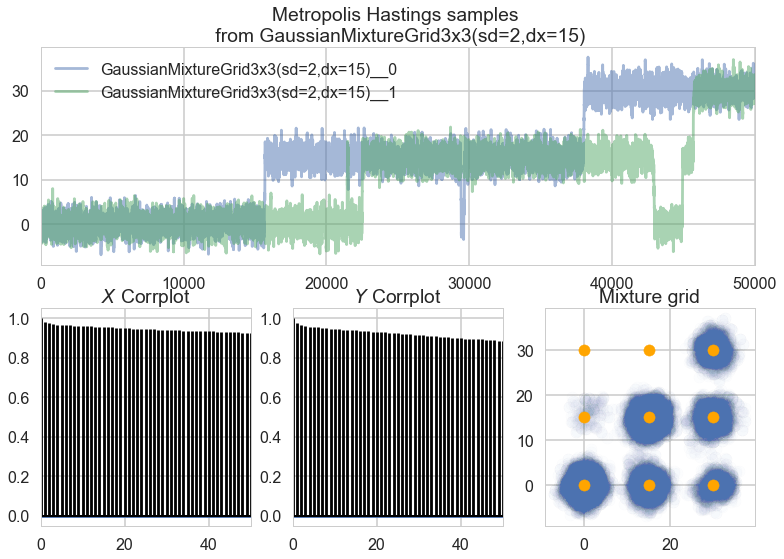
\includegraphics[width=\textwidth]{mh-trace.png}

The samples above are from a Metropolis-Hastings sampler, which is a relatively
simple MCMC technique. Note that even after removing the first 10\% of samples
from the chain and further thinning the chain by a factor of 10, there are
still very high levels of autocorrelation and the distribution of samples does
not reach all of the actual modes.   However, even Hamiltonian Monte Carlo, the
state of the art, gets stuck in similar ways:

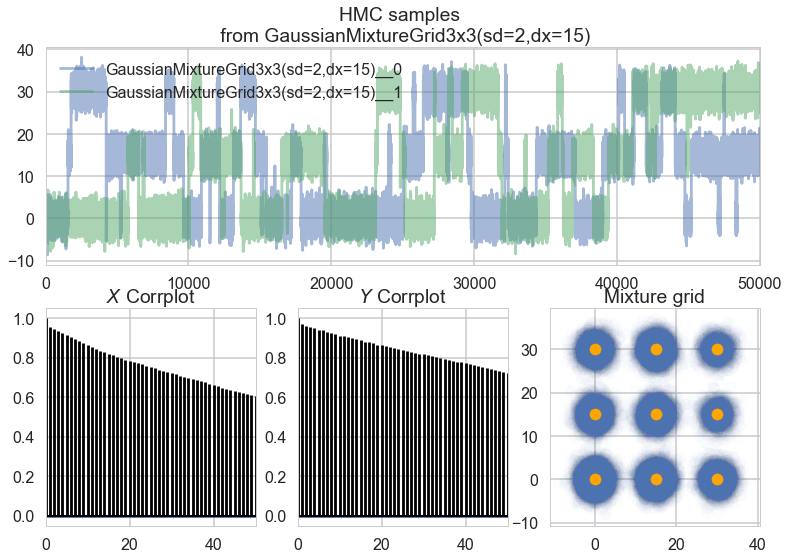
\includegraphics[width=\textwidth]{HMC-trace.png}

The crux of the problem is that for MCMC to converge, the underlying
distribution must be \textit{ergodic}. Ergodicity is a complex concept but it
intuitively corresponds to reachability; every place in the distribution must
be reachable from any other via entirely local movements. A mixture of
Gaussians like the one from which we sample above technically is ergodic,
because the density is never truly 0 anywhere. However, it is only barely
ergodic. When our distribution is not ergodic or not ergodic enough, our MCMC
samples will be inherently biased.

Because of this inherent bias, MCMC can take impractically many iterations to
converge, and furthermore, the way its convergence speeds up when combining
results from multiple parallel chains is not ideal:

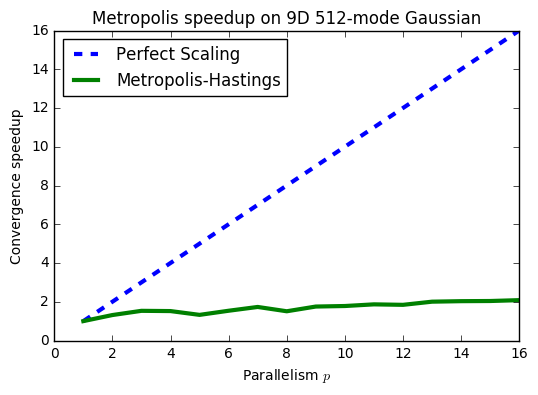
\includegraphics[width=\textwidth]{mcmc-scaling.png}

However, MCMC's advantage is that it scales well with dimensions in terms of
generating lots of samples (even if they are biased). So while MCMC may take a
long time to converge, when it does finally converge, you'll have a lot of
samples.

\subsection{Rejection Sampling}

Rejection sampling is at the opposite end of the spectrum from
Metropolis-Hastings, though it is also quite simple to describe. In rejection
sampling, you essentially draw a giant box enclosing your distribution $s$:

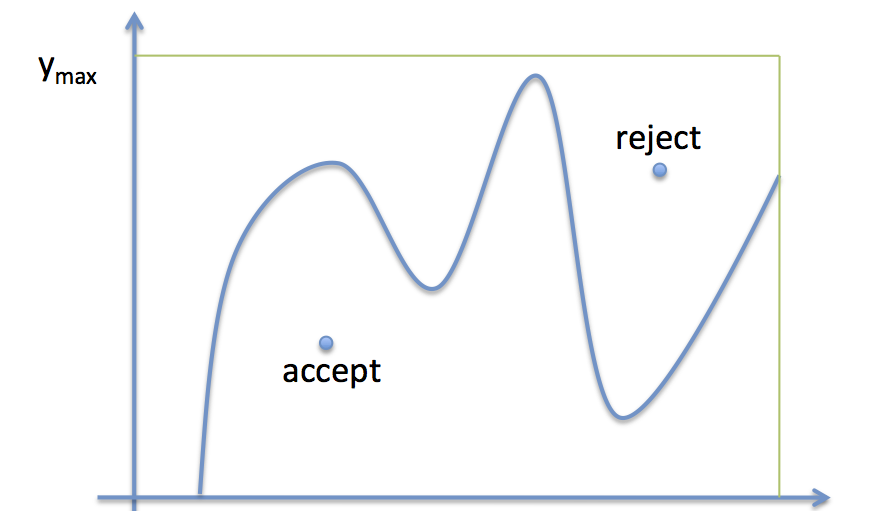
\includegraphics[width=\textwidth]{rej-illust.png}

With psuedocode:

\begin{lstlisting}[mathescape=true]
function RejectionSample($s$, N):
  samples = []
  for attempt in 1...N:
    $x, y$ $\sim$ box enclosing $s$
    if $y$ < $s(x)$:
      samples.add($x$)
  return samples
\end{lstlisting}

For distributions with infinite support, you can use an encapsulating Gaussian
or other analytically samplable distribution in place of a box, or you can
approximate one. In any case, you pick a random location within your enclosing
distribution, then check to see if it falls underneath $s$ at that
location. If so, you accept it, but otherwise, you reject it. Unlike in MCMC,
you discard the rejected samples, and the method is completely global; samples
are exactly from $s$ and entirely uncorrelated with each other (iid).

These properties make rejection sampling quite robust to multimodality. Even
with 512 fairly disconnected modes, we see a much better speedup in convergence
when combining samples from multiple rejection samplers:

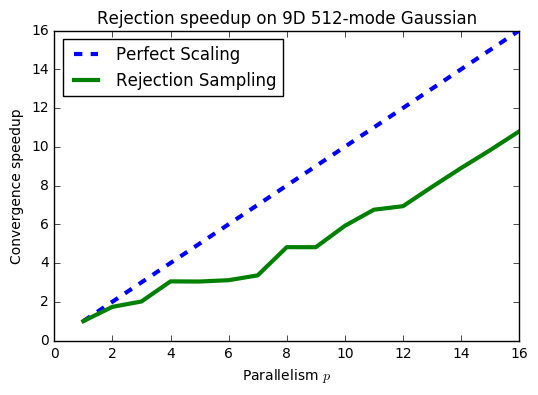
\includegraphics[width=\textwidth]{rej-scaling.png}

Furthermore, although MCMC is kind of an inherently sequential algorithm since
we must build a chain from location to location, rejection sampling can be
parallelized at every level (both across nodes using MPI and within nodes using
OpenMP).

However, although rejection sampling can handle multimodality, it can't handle
multidimensionality. The fraction of samples we accept falls exponentially as
the number of dimensions is increased (and the underlying distribution becomes
ever more sparse.) This relationship is illustrated by this Gaussian mixture
example:

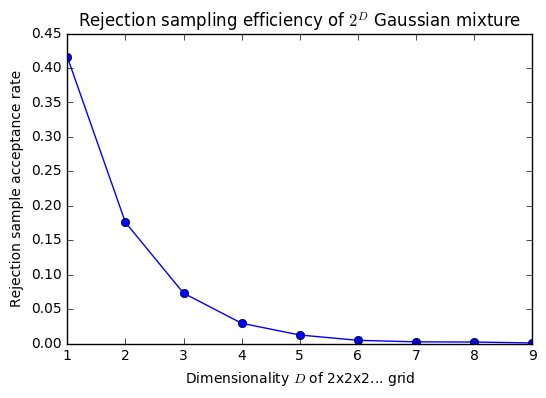
\includegraphics[width=\textwidth]{rej-dim-scaling.png}

From this analysis, we can consider rejection sampling and MCMC as two
different extremes of point-based sampling (and if we use a giant,
$s$-enclosing proposal distribution for MCMC, they become almost
equivalent). But they have exactly the opposite strengths and weaknesses: MCMC
handles dimensionality well but not multimodality; rejection sampling handles
multimodality well but dimensionality.

\section{Teleporting Hybrid}

Our main intuition is to simply linearly interpolate between rejection sampling
and MCMC. There is related work (\cite{wormhole}, \cite{darting}) which
attempts to (literally) bridge some of the gaps in MCMC, but to our knowledge,
our particular method is novel -- though perhaps only because rejection
sampling is tricky to set up and becomes inefficient so quickly.

Nevertheless, in our method, during each Metropolis-Hastings step, we either
sample from our proposal distribution with probability $1-\epsilon$ (in
which case we accept or reject using the normal MH acceptance probability) or
we ``teleport'' to a new location obtained by rejection sampling with probability
$\epsilon$. Psuedocode is as follows:

\begin{lstlisting}[mathescape=true]
function TeleportingMCMC($s$, $p$, $x_0$, N, $\epsilon$):
  samples = [$x_0$]
  attempts = 0
  while attempts < N:
    if rand(0,1) < $\epsilon$:
      repeat {
        $x, y$ $\sim$ box enclosing $s$
        attempts++
      } until y < $s(x)$
      samples.add($x$)
    else:
      $x_{1}$ = previous sample
      $x_{2} \sim p(x|x_{1})$
      attempts++
      samples.add(rand(0,1) < $s(x_{2})/s(x_{1})$ ? $x_{2}$ : $x_{1}$)
  return samples
\end{lstlisting}

In practice, we also return an array of the attempt indexes at which we
accepted each sample in order to measure convergence at any iteration.

It is straightforward to show that this scheme, expressed within the framework
of traditional Metropolis-Hastings, still satisfies the detailed balance
criteria:

$$ \frac{\text{prob of }x_1\to x_2}{\underbrace{\text{prob of }x_2\to
x_1}_{\text{must eq. $s(x_1)/s(x_2)$}}} = \frac{(1-\epsilon)p(x_1|x_2)s(x_1) +
(\epsilon) s(x_1)}{\underbrace{(1-\epsilon)p(x_2|x_1)s(x_2)}_{\text{proposal}}
+ \underbrace{(\epsilon) s(x_2)}_{\text{teleport}}} = \frac{
\big(p(x_1|x_2)(1-\epsilon) + \epsilon\big)s(x_1) }{ \big(
\underbrace{p(x_2|x_1)}_{=\, p(x_1|x_2)}(1-\epsilon) + \epsilon\big) s(x_2) } =
\underbrace{\frac{s(x_1)}{s(x_2)}}_{\text{balanced}} $$

Note also that setting $\epsilon=0$ is exactly Metropolis-Hastings, while
$\epsilon=1$ is exactly rejection sampling; we are linearly interpolating
between the two methods.

What we would like to investigate is whether, by choosing an intermediate value
for $\epsilon$, we can obtain samples that allow us to reach convergence
more quickly with better parallel scaling.

We've animated the difference between $\epsilon=0$ and $\epsilon=.0334$
here:

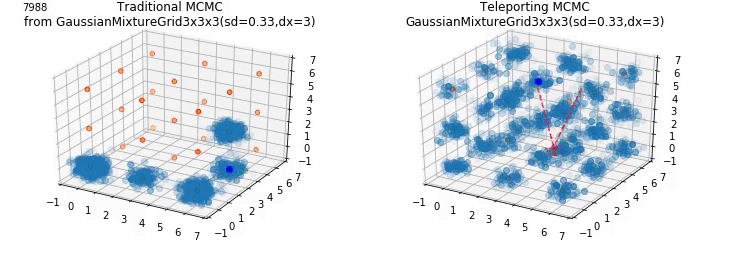
\includegraphics[width=\textwidth]{mcmc-tel-animation.png}

\section{Implementation}

\subsection{Hybrid Strategy}

The different phases in our parallelization of the problem are illustrated by
this diagram:

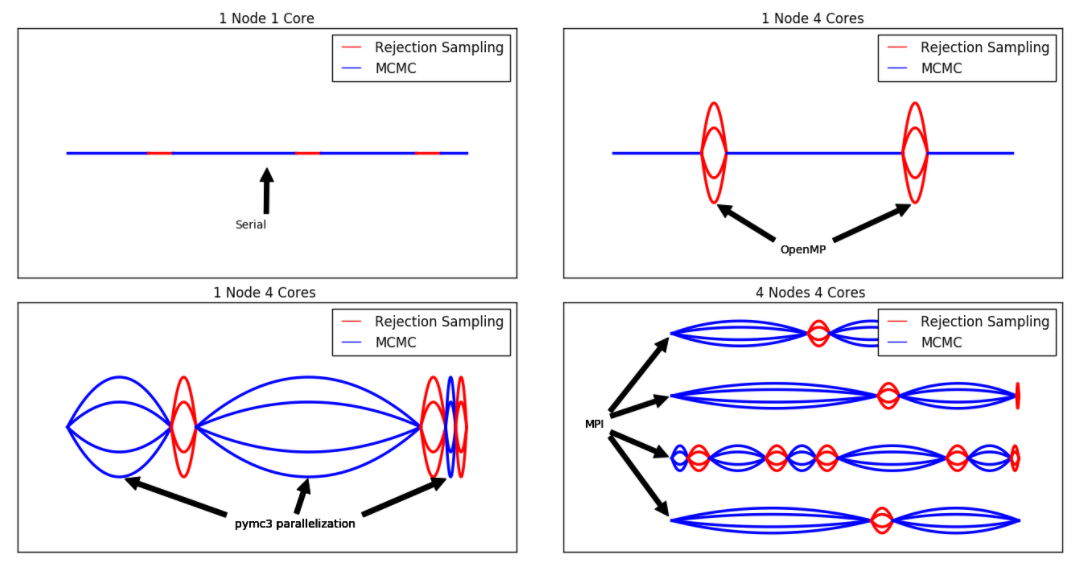
\includegraphics[width=\textwidth]{odyssey-setup.png}

Our strategy for moving from a serial (top-left) to parallel implementation
(bottom-right) is illustrated as follows. Lines represent nodes, webs represent
processors.

Teleporting MCMC consists of two alternating sampling strategies; rejection
sampling (red) and Markov chain Monte Carlo (blue). We distribute work across
processors using:

- OpenMP (via Cython) for rejection sampling; and - PyMC3's native support for
multiple jobs for Hamiltonian MC.

We distribute work across nodes using MPI, specifically using
\href{http://mpi4py.scipy.org/}{mpi4py}. Naive parallel code is available
\href{https://github.com/asross/cs205-project/blob/master/odyssey_setup/mpi_mcmc/mpi_mcmc.py}{here},
and our hybrid code (with test cases) is
\href{https://github.com/asross/cs205-project/tree/master/odyssey_setup/teleporting_mcmc2}{here}.
We also tested using OpenAcc and CUDA for GPU-based parallel rejection
sampling, which can be seen
\href{https://github.com/asross/cs205-project/tree/master/odyssey_rejection_sampling}{here}.
Note that thorough testing is slightly less important for us because we
evaluate our code via convergence metrics \ref{sec:results-conv}, which implicitly
test correctness.

\subsection{Synthetic Dataset}

The model we chose to run our experiments against is the Gaussian mixture
model.  This problem is synthetic rather than real-world, but it has the
advantage of being analytically tractable and easy to sample from, so we can
easily evaluate a number of exact rather than approximate convergence metrics.
We describe a major real-world application later on \ref{sec:relwork-sens}. Here are
contour plots of the density of a 2D, 3x3 Gaussian mixture grid:

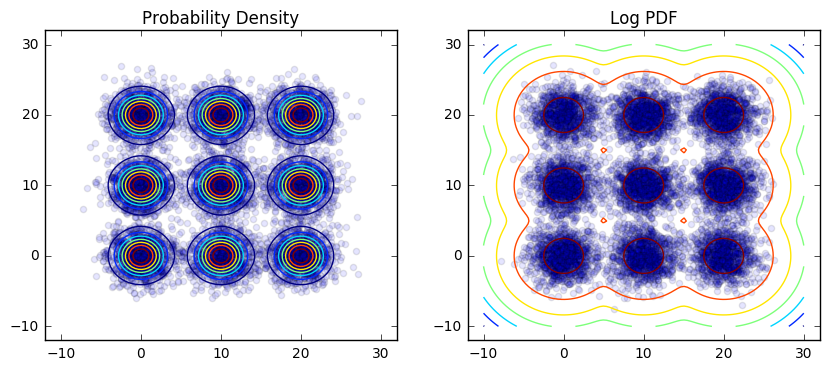
\includegraphics[width=\textwidth]{pdf-and-log-pdf.png}

We implemented a \href{https://github.com/asross/cs205-project/blob/master/datasets/gaussian_mixture_grid.py}{parameterized class}
to generate Gaussian mixtures with varying dimensions, spacing, variance, and
mode count:

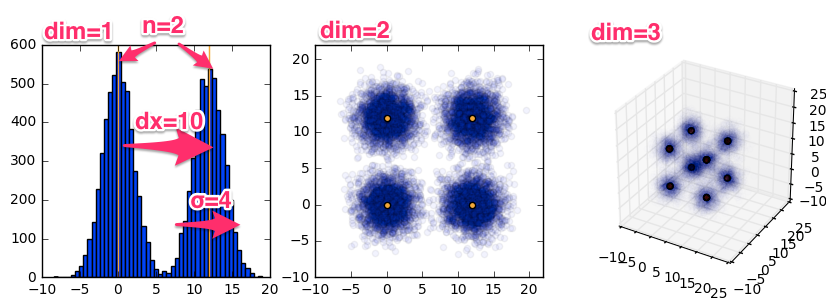
\includegraphics[width=\textwidth]{gmixgrid.png}

This gives us the flexibility to increase the multimodality and variance of our
distribution while keeping the distribution tractable enough to accurately
assess convergence.

\section{Results}

\subsection{Which Method is Best?}

The short answer? It depends (especially on dimensionality):

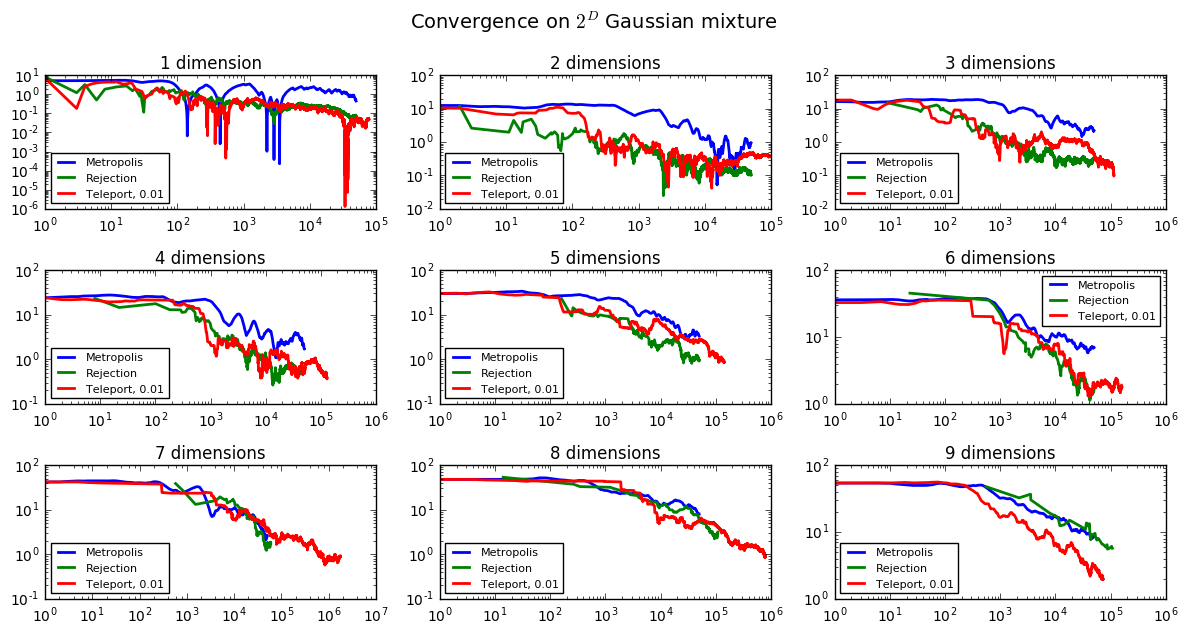
\includegraphics[width=\textwidth]{which-meth-best.png}

These results are for a grid with $2^\text{number of dimensions}$ modes
with a grid spacing of 25, and with each mode having a standard deviation of 4.
Our teleporting algorithm is always at least as good as the best method, but
it's not until we reach very high dimensions -- 9, which corresponds to
$2^9=512$ modes -- that it starts to outperform both the metropolis and
rejection samplers.

Those were plots for individual chains, but the main item of interest is how
the results change with parallelism. Let's examine how the number of iterations
until we reach a particular level of convergence (implementation details
below \ref{sec:results-conv}) changes as we vary the number of \textit{parallel} runs (note:
these results are using our naive parallel implementation that does not
parallelize the rejection sampling portion):

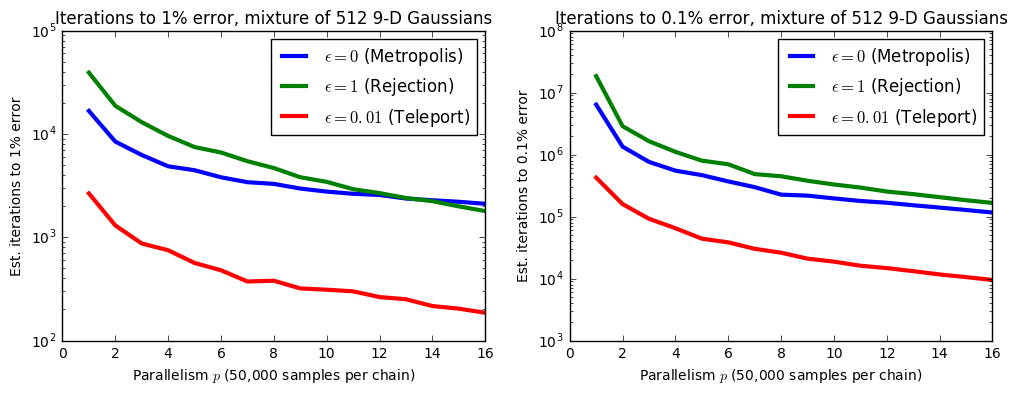
\includegraphics[width=\textwidth]{time2tol.png}

From these plots, the advantage of the teleporting sampler is clear, but what
is also interesting is the difference in scaling behavior between the
teleporting sampler and unaided Metropolis-Hastings (as well as how it varies
with the tolerance). Because of the independence of its samples, rejection
sampling is better able to exploit parallel resources even though its
efficiency at 9 dimensions is only $\approx 0.0008$ -- less than one tenth
of one percent. Metropolis isn't significantly helped by having more parallel
chains because each chain is individually biased; they need to reach a minimum
length before they fully contribute. Our teleporting sampler appears to get the
best of both worlds; it only needs to rejection sample about every 100
iterations, but it's fairly unbiased, so it scales well.

When we need to reach a higher degree of precision, Metropolis-Hastings starts
doing a little better compared to rejection sampling, even though the gap does
start narrowing as we increase $p$. Perhaps this is because the number of
iterations per chain is several orders of magnitude higher, so each chain is
closer to mixing.

\subsection{Scaling vs. \(\epsilon\)}

Independently of inter-method differences, we can also analyze intra-method
speedups (moving back into linear from log space):

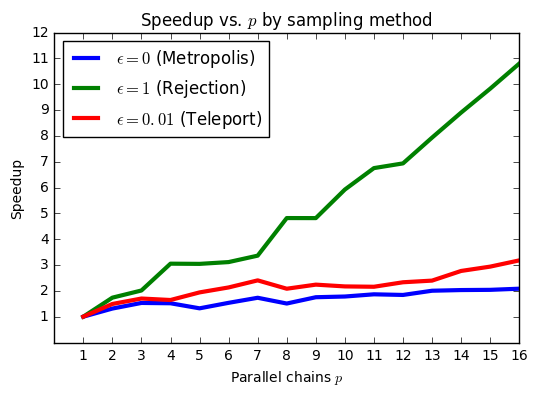
\includegraphics[width=\textwidth]{speedup-comp.png}

We included some of these results above in the background section because they
felt useful not just as results but as characterizations of the methods
themselves. Essentially, rejection sampling is serving as the gold standard: it
produces uncorrelated samples, and so we should expect near-perfect speedup
(almost equaling $p$). Metropolis produces highly correlated samples, so we
should expect a much less significant speedup from parallelization. Finally,
the teleportation method should be somewhere in between (which it is). Given a
particular time vs. parallelism cost tradeoff, we should be able to choose a
cost-optimal $\epsilon$ for our sampler to reach a particular level of
precision.

Why not perfect speedup for rejection sampling? As we explain
below \ref{sec:results-conv}, these speedups are essentially measuring reduction in a
standard deviation that depends both on the inefficiency of the sampler and on
the underlying variance of the distribution. As we increase $p\to\infty$,
we expect the inefficiency of rejection sampling to go away completely since
the samples are fully iid. However, there will still be an underlying variance
inherent to the \textit{distribution}, which will remain constant -- essentially a
minimum problem size.

We feel there may be interesting theoretical connections between ideas about
overhead in parallel systems to variance in probabilistic ones.

\subsection{Speedups on Odyssey}

First, using MPI (code
\href{https://github.com/asross/cs205-project/blob/master/odyssey_setup/mpi_mcmc/mpi_mcmc.py}{here},
we find we are able to run many, many parallel chains (up to 128)
simultaneously. Our results show that for a fixed problem size we can achieve
higher speedups by increasing the number of processors. The efficiency starts
to drop with more processors, and thus MPI alone does not quite achieve strong
scaling. However, for a fixed number of processors we can maintain a similiar
efficiency for larger problem sizes.

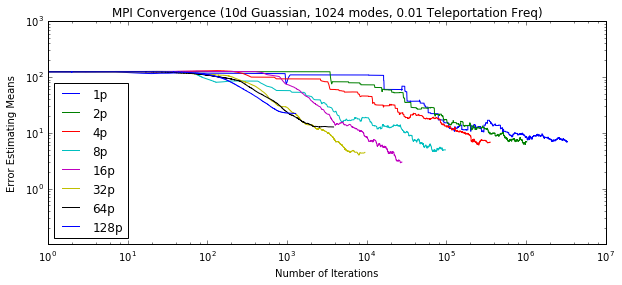
\includegraphics[width=\textwidth]{mpi-conv.png}
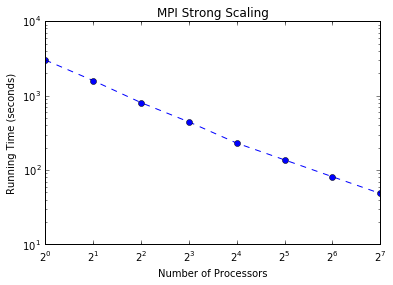
\includegraphics[width=\textwidth]{mpi-strong-scale1.png}
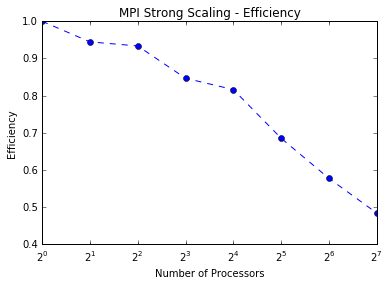
\includegraphics[width=\textwidth]{mpi-strong-scale2.png}
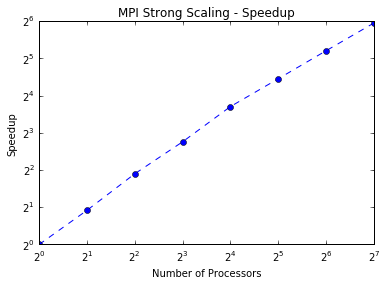
\includegraphics[width=\textwidth]{mpi-strong-speedup.png}
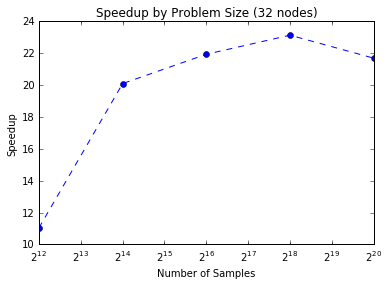
\includegraphics[width=\textwidth]{mpi-speedup-sample.png}

These are just results for the naive parallel case using MPI. We pursued a
hybrid approach to decrease the amount of MPI communication. We considered both
OpenMP (code
\href{https://github.com/asross/cs205-project/blob/master/odyssey_rejection_sampling/openmp_dir/openmp.c}{here})
and OpenAcc (code
\href{https://github.com/asross/cs205-project/blob/master/odyssey_rejection_sampling/openacc_dir/openacc.cpp}{here}):

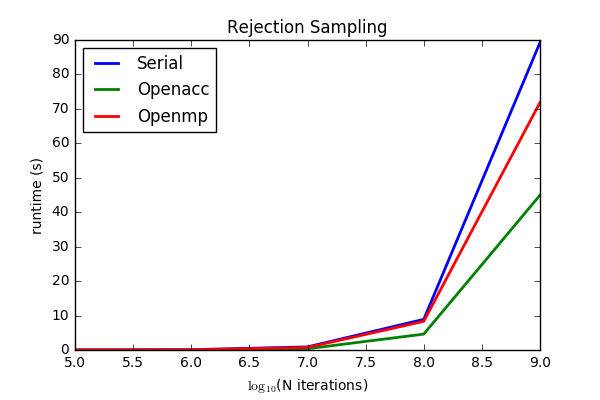
\includegraphics[width=\textwidth]{openaccmp.png}

Although OpenACC is clearly somewhat faster, we settled on OpenMP for two
reasons:

1. Generating random numbers within kernels is non-trivial. A naive approach
would have each thread spin random numbers off a different seed. However, some
random number generators fail to give independent sequences with different
seeds which is particularly problematic when so many threads are involved. CUDA
offers cuRAND to deal with randomness in a sophisticated manner and a bare
bones implementation of rejection sampling using cuRAND is available in the
repo. However with OpenACC the convention is to generate random numbers on the
host and pass them to the device. This leads to increased communication
overhead in terms of memory and time and impairs gains from harnessing the GPU.

2. Ease of integration with the Python framework (which housed the rest of our
code).

Below are our full hybrid results for speedup (final code
\href{https://github.com/asross/cs205-project/blob/master/odyssey_setup/teleporting_mcmc2}{here}):

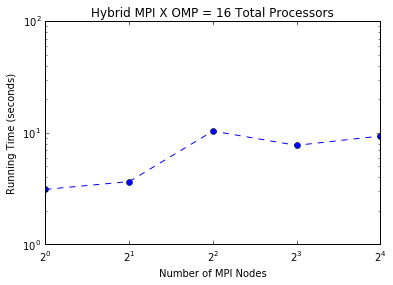
\includegraphics[width=\textwidth]{hybrid-results.png}

This plot is for 16 total processors/nodes which we allocate between MPI and
OpenMP. The lowest runtime (the first dot) is when we allocate all of our
processing power to OpenMP, suggesting that OpenMP is giving us the most bang
for its buck on Odyssey. Clearly, given infinite parallel resources, we should
use both OpenMP and MPI.

\subsection{Convergence Details}

First, using MPI (code
\href{https://github.com/asross/cs205-project/blob/master/odyssey_setup/mpi_mcmc/mpi_mcmc.py}{here},
we find we are able to run many, many parallel chains (up to 128)
simultaneously. Our results show that for a fixed problem size we can achieve
higher speedups by increasing the number of processors. The efficiency starts
to drop with more processors, and thus MPI alone does not quite achieve strong
scaling. However, for a fixed number of processors we can maintain a similiar
efficiency for larger problem sizes.

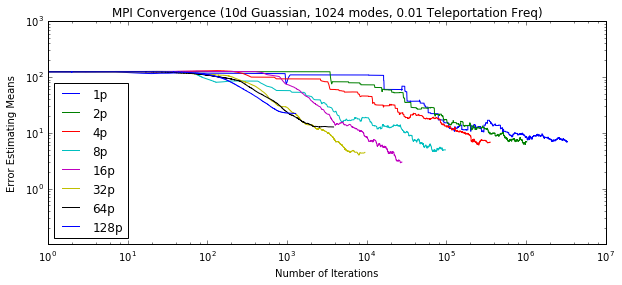
\includegraphics[width=\textwidth]{mpi-conv.png}
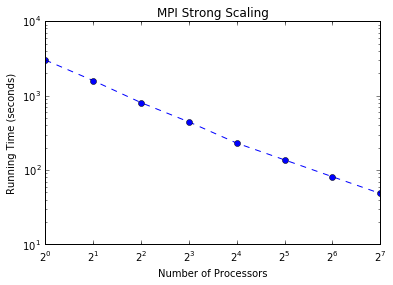
\includegraphics[width=\textwidth]{mpi-strong-scale1.png}
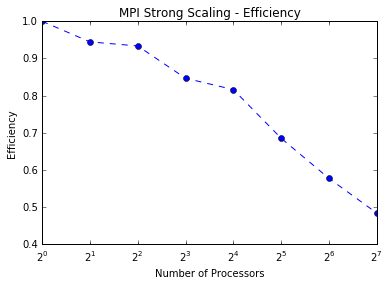
\includegraphics[width=\textwidth]{mpi-strong-scale2.png}
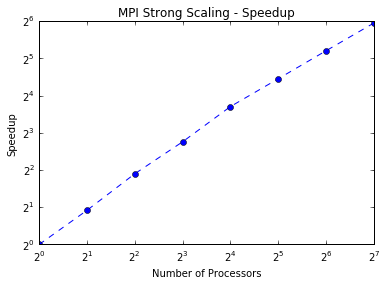
\includegraphics[width=\textwidth]{mpi-strong-speedup.png}
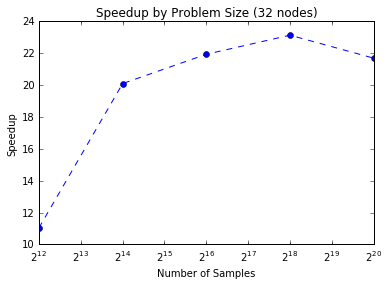
\includegraphics[width=\textwidth]{mpi-speedup-sample.png}

These are just results for the naive parallel case using MPI. We pursued a
hybrid approach to decrease the amount of MPI communication. We considered both
OpenMP (code
\href{https://github.com/asross/cs205-project/blob/master/odyssey_rejection_sampling/openmp_dir/openmp.c}{here})
and OpenAcc (code
\href{https://github.com/asross/cs205-project/blob/master/odyssey_rejection_sampling/openacc_dir/openacc.cpp}{here}):

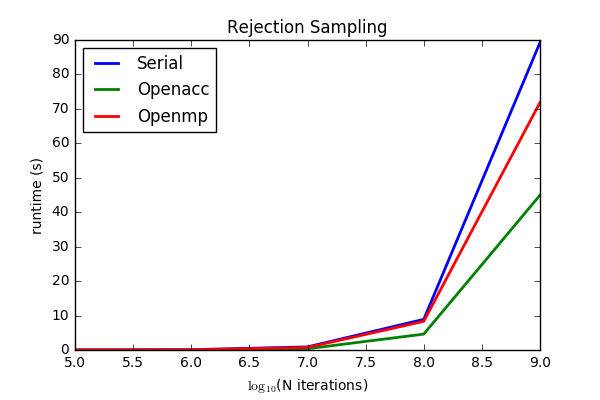
\includegraphics[width=\textwidth]{openaccmp.png}

Although OpenACC is clearly somewhat faster, we settled on OpenMP for two
reasons:

1. Generating random numbers within kernels is non-trivial. A naive approach
would have each thread spin random numbers off a different seed. However, some
random number generators fail to give independent sequences with different
seeds which is particularly problematic when so many threads are involved. CUDA
offers cuRAND to deal with randomness in a sophisticated manner and a bare
bones implementation of rejection sampling using cuRAND is available in the
repo. However with OpenACC the convention is to generate random numbers on the
host and pass them to the device. This leads to increased communication
overhead in terms of memory and time and impairs gains from harnessing the GPU.

2. Ease of integration with the Python framework (which housed the rest of our
code).

Below are our full hybrid results for speedup (final code
\href{https://github.com/asross/cs205-project/blob/master/odyssey_setup/teleporting_mcmc2}{here}):

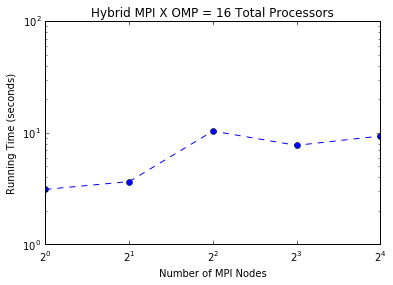
\includegraphics[width=\textwidth]{hybrid-results.png}

This plot is for 16 total processors/nodes which we allocate between MPI and
OpenMP. The lowest runtime (the first dot) is when we allocate all of our
processing power to OpenMP, suggesting that OpenMP is giving us the most bang
for its buck on Odyssey. Clearly, given infinite parallel resources, we should
use both OpenMP and MPI.

\section{Related Work}

\subsection{Other Methods}

Other methods exist for sampling from multimodal distributions. A simple one is
the idea of random restarts \cite{restarts}, where we start multiple chains at
uniformly random points in state space, but weight the samples from each chain
by the density at those random starting locations. This approach is similar in
spirit to teleportation, except teleportation implicitly accounts for the
downweighting by rejection sampling from the distribution itself, rather than
uniformly. I believe for random restarts, also, the length of each chain is
constant, whereas in teleportation it is random. Future work should investigate
to what extent these methods are similar; given that rejection sampling is much
less likely to place our chain in a region of near 0 probability, it is
possible that random restarts will do a worse job of efficiently sampling the
multimodal typical set than teleportation.

A more complex idea is parallel tempering, where we generate multiple replicas
of an MCMC chain that each behave differently. In particular, each chain
operates at a different "temperature," which determines the likelihood of
sampling from a low probability region in the distribution of interest.
Parallel tempering facilitates exploration by allowing each chain, operating at
a different temperature, to exchange complete configurations. That is, chains
operating at low temperatures can access regions more readily available to
chains running at high temperatures. This has been found to converge much
faster than vanilla MCMC, but tuning temperature values for each chain can be
difficult. Moreover, the algorithm may not scale well, because the procedure
for swapping states is sensitive to the overlap in search between those two
states. It would be interesting to compare this with our method, or even to
investigate combining them.

We almost neglected to mention Hamiltonian Monte Carlo \cite{hmc} because it is
so ubiquitous; it is a major improvement on top of normal Metropolis-Hastings
that is able to sample high-dimensional distributions much more efficiently by
utilizing local gradient information about the probability distribution.
Although HMC is efficient at overcoming "low energy barriers" in partially
multimodal problems, where modes are separate but still connected by regions of
nonzero probability, HMC suffers from the same issues as Metropolis-Hastings in
sampling truly multimodal distributions (which we might expect for any
gradient-based method faced with nonconvexity). Hamiltonian Monte Carlo should
not be seen as a competitor to our method; for ease of implementation, we
implemented our teleportation algorithm on top of Metropolis-Hastings, but for
future work, we would implement HMC with teleportation to make the local
sampling steps more efficient.

Finally, we should mention other attempts to improve on HMC. Wormhole
Hamiltonian Monte Carlo \cite{wormhole} adds auxiliary dimensions to the normal
problem of sampling to create a "mirror world." Within this augmented mirror
world, normally disconnected modes become close in proximity in the auxiliary
dimension. Modes are connected in a network. For simple problems, the modes can
specified beforehand, but in general Wormhole HMC attempts to discover them
during normal HMC with random restarts. This complicates the implementation of
the algorithm and still produces biased results if all modes are not
discovered. However, after they are, Wormhole HMC samples extremely
efficiently.

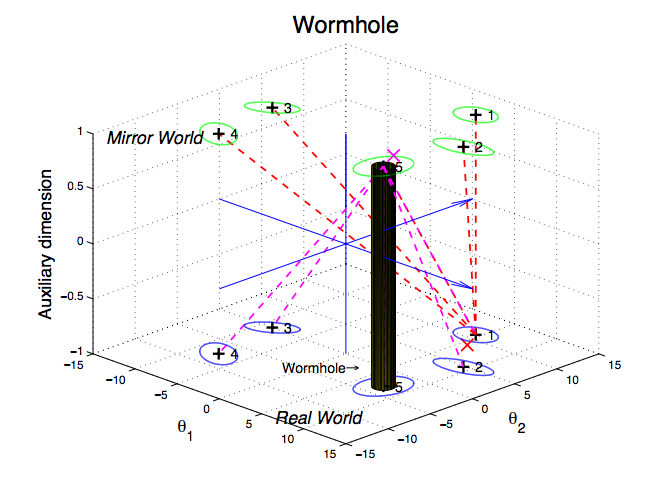
\includegraphics[width=\textwidth]{wormholehmc.png}

\subsection{Application: Noisy Sensors}

One real-world application to which we can directly apply our method is sensor
localization, which is discussed by both \cite{wormhole} and \cite{darting}.

The setup for this problem is as follows. Assume we have a collection of
$N$ sensors with 2D or 3D locations $\vec{x}_k$ which noisily attempt
to communicate with each other. For any pair of sensors $i$ and $j$,
there is an exponentially decreasing probability they can communicate at all,
indicated by

$$ Z_{ij} \sim \text{Bern}\left(\exp\left(\frac{-||\vec{x}_i -
\vec{x}_j||^2}{2R^2}\right)\right) $$

Assuming $Z_{ij} = 1$, i.e. that they \textit{do} manage to communicate, they
transmit a noisy measurement of their distance

$$ Y_{ij}|(Z_{ij} = 1) \sim \mathcal{N}\left(||\vec{x}_i - \vec{x}_j||,
\sigma^2\right) $$

where $R$ and $\sigma$ are known sensor parameters. The total
probability of observing our data $Y$ and $Z$ given our locations
$\vec{x}$ is just the product of all of these terms for each $i, j$
pair.

In general we are interested in the reverse problem; we have the measurement
data but do not know the sensor locations. However, assuming a uniform prior on
the sensor locations, the probability of the locations given the data is
proportional to the probability of the data given the locations. For both MCMC
and rejection sampling, this is enough; we do not need to know the normalizing
constant of our distribution, just its relative density at each location.

In general (as you might imagine), the resulting posterior distributions of
sensor locations given measurement data are often multimodal, sometimes with
many different modes for each sensor. In the case below, which is for $N=8$
on a 2D grid (with three extra sensors with known locations, to resolve mirror
symmetry ambiguities), we have a 16-dimensional posterior distribution of the
$x,y$ locations of each sensor, whose marginals are projected onto a 2D
plane (with true locations represented as circles):

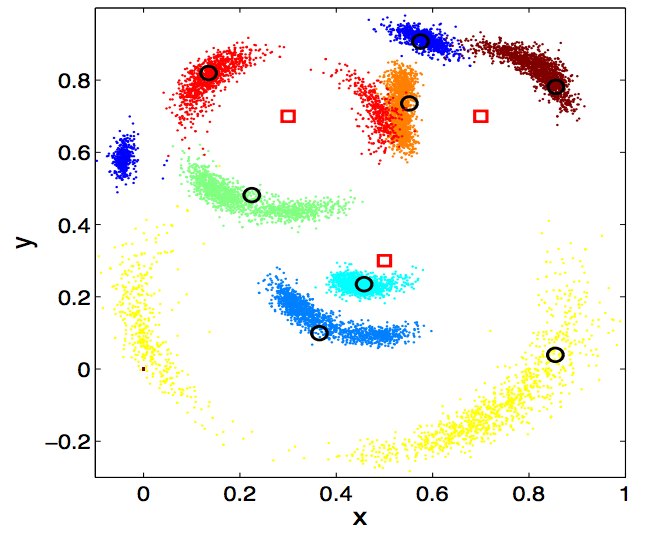
\includegraphics[width=\textwidth]{noisysensor.png}

As you can see, there is true multimodality to this real-world problem, with
multiple valid hypotheses for the locations of many sensors, which, as
\cite{wormhole} shows, many state of the art MCMC methods fail to adequately
capture. Given additional time, it would be straightforward to apply our method
to this problem, and we believe it could be competitive with the algorithms
presented in \cite{wormhole} and \cite{darting}, especially if $\epsilon$
is tuned to optimize parallel resources.

\subsection{Connections to PageRank}

As a brief aside, our method has some interesting connections to PageRank
\cite{pagerank}, an enormously successful MCMC algorithm that Google used to
determine a sensical popularity-based order of pages on the web. It essentially
operates by doing a random walk over the entire web and ranking pages based on
how often they are visited.

The issue is that there are disconnected subgraphs in the web (which are kind
of like a discrete analogue to multimodality or non-convexity in a probability
distribution), which makes the random walk impossible. This means that the
standard method for running MCMC over discrete graphs, the power iteration
(which essentially just extracts eigenvalues corresponding to the final ranks
via a series of matrix multiplications -- almost a classic parallel algorithm),
doesn't work. The transition matrix is singular. PageRank resolves this by
adding a small "teleportation" term which essentially adds a chance of jumping
to an entirely random page at any point in the random walk. Schematically, this
can be illustrated as follows:

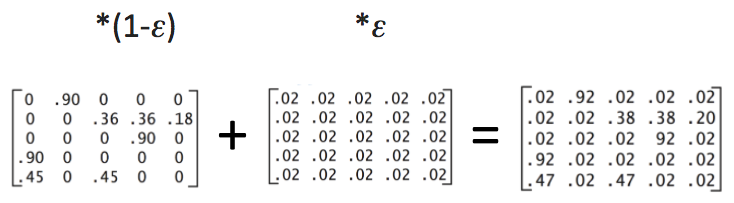
\includegraphics[width=\textwidth]{pagerank-mat.png}

Or in graph form:

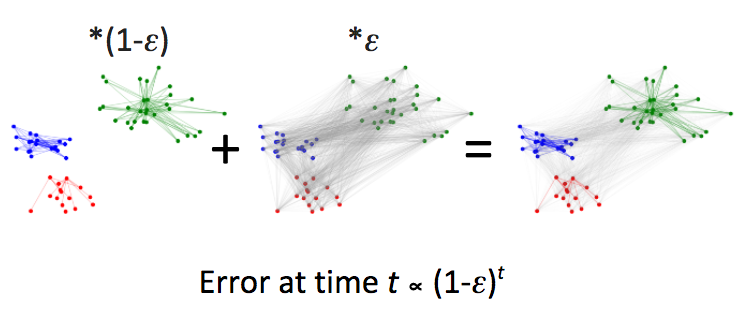
\includegraphics[width=\textwidth]{pagerank-graph.png}

The resulting matrix is no longer singular, although its condition number will
be high and convergence will be slow if $\epsilon$ is too small (see
\cite{convspeed} and \cite{secondeig}). If $\epsilon$ is too high, then the
distribution becomes uniform and the distinction between pages blurs. But there
is a happy medium where the problem is well-conditioned, converges quickly, and
the results provide a meaningful ranking of pages.

This simple discrete example has close conceptual connections to our approach
on sampling. Instead of a discrete but disconnected graph, we have a multimodal
probability distribution, and again we speed up the inherent convergence
properties of our MCMC algorithm by adding a small probability of teleportation
everywhere. Unlike PageRank, increasing $\epsilon$ does not change the
distribution, because our teleportation uses rejection samples from the
probability distribution itself, but it does come at the cost of a
computationally inefficient process to obtain the next rejection sample. This
problem is of interest in this class in particular because our tradeoff also
involves a change in the parallel scaling behavior of the algorithm.

\section{Conclusions}

\subsection{Checking the Boxes}

To summarize, in this project we have:

\begin{itemize}

\item Devised a novel sampling method for intractable multimodal
  distributions, which arise in problems like sensor localization and topic
  modeling.

\item Investigated the parallel scaling properties inherent to both the
  algorithm and the problem, with particular focus on the sampling efficiency
  vs. parallel scaling tradeoffs.

\item  Implemented both naive and hybrid parallel versions of our algorithm
  using MPI, OpenMP, OpenAcc, and multi-process parallelelism, demonstrating
  strong scaling along the way.

\end{itemize}

\subsection{Discussion and Future Work}

One main thing we would attempt to determine next would be the (cost or time)
optimal $\epsilon$ for a given distribution and set of parallel resources.
We have demonstrated that, at the very least, neither $\epsilon=0$ nor
$\epsilon=1$ is optimal for a high dimensional Gaussian mixture model, but
we have not found the best value.

Another complexity that should be analyzed is how much our method of
parallelizing rejection sampling (within each MPI node) affects this optimal
$\epsilon$. Because of this strong coupling between parallel scaling and
$\epsilon$, improving the parallelism of our algorithm could potentially
mean that we must choose a higher value if we want to reach a specified
convergence threshold in a cost-optimal manner.

Finally, we would like to shore up our theoretical analysis of the relationship
between the variance of the distribution and the scaling properties of
samplers. In general, we think there is value in trying to bridge the
conceptual gaps between parallel computing and statistics, optimization, and
numerical methods, which are subjects we have all been studying ``in parallel''
in the CSE program. We hope that by sampling all of these academic modes
together, with plenty of jumping back and forth, we can ultimately converge on
better solutions to the big science problems that motivate them all.

\small
\bibliographystyle{plain}
\bibliography{bibliography}

\end{document}
